% arXiv categories: cs.AI (primary), cs.CL (secondary)
% arXiv identifier: [to be assigned]
\pdfoutput=1
\documentclass[11pt,letterpaper]{article}

% ============================================================
% PACKAGES
% ============================================================
\usepackage[utf8]{inputenc}
\usepackage[T1]{fontenc}
\usepackage{lmodern}
\usepackage[margin=1in,top=1.25in]{geometry}
\usepackage{graphicx}
\usepackage{booktabs}
\usepackage{array}
\usepackage{amsmath}
\usepackage{amssymb}
\usepackage{amsthm}
\usepackage{enumitem}
\usepackage{xcolor}
\usepackage{listings}
\usepackage{tikz}
\usepackage{algorithm}
\usepackage{algpseudocode}
\usepackage{float}
\usepackage{placeins}
\usepackage{natbib}
\usepackage{microtype}
\usepackage{fancyhdr}
\usetikzlibrary{shapes,arrows,positioning,fit,backgrounds,calc}

% hyperref loaded last
\usepackage[bookmarks=true,breaklinks=true]{hyperref}
\usepackage{url}

% ============================================================
% PAGE BREAK CONTROL
% ============================================================
\widowpenalty=10000
\clubpenalty=10000
\raggedbottom

% ============================================================
% THEOREM ENVIRONMENTS
% ============================================================
\newtheorem{definition}{Definition}[section]
\newtheorem{theorem}{Theorem}[section]
\newtheorem{lemma}[theorem]{Lemma}
\newtheorem{proposition}[theorem]{Proposition}

% ============================================================
% CUSTOM TITLE FORMATTING (NeurIPS-like)
% ============================================================
\makeatletter
\def\@maketitle{%
  \newpage
  \null
  \vskip 0.5em%
  {\centering
    \rule{\textwidth}{1.5pt}\\[0.4em]
    {\LARGE\bfseries \@title \par}%
    \vskip 0.4em%
    \rule{\textwidth}{0.4pt}\\[1.5em]
    \@author\par
  }%
  \vskip 1.5em}
\makeatother

% Abstract styling
\renewenvironment{abstract}{%
  \vskip 1em%
  \begin{center}%
    \bfseries Abstract%
  \end{center}%
  \begin{quotation}%
    \small\noindent
}{%
  \end{quotation}%
  \vskip 1em%
}

% Footer with page numbers
\pagestyle{fancy}
\fancyhf{}
\renewcommand{\headrulewidth}{0pt}
\fancyfoot[C]{\thepage}

% ============================================================
% STYLING
% ============================================================
\hypersetup{
    colorlinks=true,
    linkcolor=blue!70!black,
    urlcolor=blue!70!black,
    citecolor=blue!70!black,
    pdftitle={Epistemic Augmented Generation: A Tiered Epistemology for Agent Memory},
    pdfauthor={Aliasgar Khimani},
    pdfkeywords={agent memory, epistemology, belief revision, RAG, knowledge graphs}
}

\lstset{
    basicstyle=\ttfamily\small,
    breaklines=true,
    frame=single,
    backgroundcolor=\color{gray!10}
}

% ============================================================
% DOCUMENT
% ============================================================
\begin{document}

% ------------------------------------------------------------
% TITLE
% ------------------------------------------------------------
\title{Epistemic Augmented Generation:\\A Tiered Epistemology for Agent Memory}

\author{
    \textbf{Aliasgar Khimani}\thanks{\texttt{aliasgar.khimani@engrammic.ai}}\\
    Engrammic Labs
}

\date{}

\maketitle

% ------------------------------------------------------------
% ABSTRACT
% ------------------------------------------------------------
\begin{abstract}
Retrieval-Augmented Generation (RAG) treats memory as a retrieval problem: store content, embed it, fetch what's relevant. This works for static knowledge bases but fails for agents that learn over time, where memories contradict, beliefs evolve, and corrections must propagate. RAG commits a \textit{category error}: applying uniform persistence semantics to information with fundamentally different epistemic status.

We introduce \textbf{Epistemic Augmented Generation (EAG)}, a paradigm that treats agent memory as an epistemology problem. Building on Roynard's identification of the missing knowledge layer in cognitive architectures, EAG formalizes stratified epistemic types with distinct evidence requirements: observations require no justification, claims require single sources, facts require corroboration, and beliefs require derivation chains. We prove our revision protocol satisfies AGM belief revision postulates and that coherence is decidable for finite stores.

We present \textbf{CITE (Context In Tiered Epistemology)}, a four-layer architecture implementing EAG: Memory for observations (decay-based), Knowledge for verified claims (supersession-based), Wisdom for synthesized beliefs (evidence-gated revision), and Intelligence for active reasoning (session-scoped). Write-time validation gates every entry by epistemic layer, preventing contradiction accumulation at the source rather than detecting it after the fact.

On contradiction detection, CITE achieves 95\% accuracy compared to 66\% for retrieval-only baselines; on revision propagation, 87\% vs 12\%. We discuss extensions to latent-space epistemology for JEPA-style world models. The architecture and implementation are open source under Apache 2.0.
\end{abstract}

% ------------------------------------------------------------
% 1. INTRODUCTION
% ------------------------------------------------------------
\section{Introduction}

RAG was built for chatbots. A user asks a question, the system retrieves relevant documents, the LLM synthesizes an answer. The documents don't change. The user doesn't correct the system. Each conversation starts fresh.

Agents are different. An agent that runs for months accumulates knowledge. It learns that the API uses OAuth2 on Monday, then learns it uses API keys on Tuesday. It stores a hallucinated fact, retrieves it next week, and treats it as ground truth. It receives a correction from the user but never propagates it to the beliefs derived from the original error.

Roynard\footnote{\url{https://arxiv.org/abs/2604.11364}}~\cite{roynard2026} identifies this as a \textit{category error}: RAG and naive memory systems apply one persistence model (typically decay) uniformly to information with fundamentally different persistence semantics. A decaying Slack message is correct; a decaying validated fact is a bug. This critique extends to cognitive architectures like CoALA\footnote{\url{https://arxiv.org/abs/2309.02427}}~\cite{sumers2023coala} and JEPA~\cite{lecun2022path}, which lack an explicit Knowledge layer with proper epistemic semantics.

\textbf{Epistemic Augmented Generation (EAG)} reframes agent memory as an epistemology problem:
\begin{itemize}[noitemsep]
    \item What do I believe? (epistemic types)
    \item Why do I believe it? (justification and provenance)
    \item How confident am I? (warrant function)
    \item What would change my mind? (revision protocol)
\end{itemize}

\subsection{Contributions}

This paper makes four contributions:
\begin{enumerate}[noitemsep]
    \item \textbf{EAG formal framework} extending Roynard's four-layer proposal with formal definitions of epistemic types, warrant functions, and coherence invariants. We prove our revision protocol satisfies AGM belief revision postulates (Theorem~\ref{thm:agm}).
    \item \textbf{CITE architecture} implementing EAG with write-time coherence enforcement, supersession chains, and dependency propagation.
    \item \textbf{Evaluation} on contradiction detection (95\% vs 66\%) and revision propagation (87\% vs 12\%) using 500 annotated coding agent sessions.
    \item \textbf{Open-source implementation} under Apache 2.0.\footnote{Code and data: \url{https://github.com/engrammic-ai/engrammic}}
\end{enumerate}

Section~\ref{sec:background} reviews formal epistemology and agent memory systems. Section~\ref{sec:eag} presents the EAG formal framework. Section~\ref{sec:cite} describes the CITE architecture. Section~\ref{sec:eval} evaluates the system. Section~\ref{sec:discussion} discusses extensions to JEPA and multi-agent systems.

% ------------------------------------------------------------
% 2. BACKGROUND
% ------------------------------------------------------------
\section{Background}
\label{sec:background}

\subsection{Formal Epistemology}

Epistemology studies knowledge: what it is, how we acquire it, how we justify it. Gettier~\cite{gettier1963} showed that justified true belief is insufficient for knowledge---lucky guesses can satisfy JTB without constituting knowledge. This motivates stronger conditions.

Plantinga~\cite{plantinga1993} introduced \textit{warrant}: the property that distinguishes knowledge from mere true belief. Warrant requires proper function of cognitive faculties, a suitable environment, and a design plan aimed at truth. We operationalize warrant as a function of evidence credibility, independence, and recency.

BonJour~\cite{bonjour1985} defends \textit{coherentism}: justification comes from membership in a coherent system of beliefs, not from foundational beliefs. Our coherence invariants implement this structurally---contradictions are rejected at write time.

\subsection{Belief Revision}

The AGM framework~\cite{agm1985} formalizes rational belief change through three operations: expansion (adding beliefs), contraction (removing beliefs), and revision (adding beliefs while maintaining consistency). Key postulates include:
\begin{itemize}[noitemsep]
    \item \textbf{Recovery}: $(K * \neg\phi) + \phi \vdash K$ (original beliefs recoverable)
    \item \textbf{Inclusion}: $K + \phi \subseteq K * \phi$ (revision doesn't lose unrelated beliefs)
\end{itemize}

We prove (Theorem~\ref{thm:agm}) that EAG's supersession operation satisfies these postulates.

\subsection{Agent Memory Systems}

Current agent memory systems lack epistemic structure:

\textbf{mem0}\footnote{\url{https://github.com/mem0ai/mem0}}~\cite{mem0} achieves 94.4\% on LongMemEval at 6.9k tokens but uses ADD-only architecture. Production failures are documented: Issue \#4573 reports 97.8\% junk rate with 808 duplicates; Issue \#4896 (closed ``not planned'') shows semantic contradictions cannot be resolved; Issue \#5330 shows no stale memory decay.

\textbf{Zep/Graphiti}\footnote{\url{https://github.com/getzep/graphiti}}~\cite{graphiti2025} implements bi-temporal validity (created\_at, valid\_at, invalid\_at) with LLM-based edge invalidation and provenance to source episodes. However, it lacks epistemic layering and evidence-gated promotion.

\textbf{MemGPT}\footnote{\url{https://github.com/cpacker/MemGPT}}~\cite{memgpt2023} provides tiered working/archival memory inspired by operating systems but without epistemic distinction between memory types.

\textbf{Hindsight}\footnote{\url{https://github.com/vectorize-io/hindsight}}~\cite{hindsight} uses four memory networks (World, Experience, Opinion, Observation) with on-demand synthesis. Gap: no live truth maintenance or dependency propagation.

\subsection{LLM Reliability Research}

Recent work identifies mechanisms that EAG addresses:

\textbf{State contamination}~\cite{wang2026contamination}: Toxic content survives compression below classifier thresholds (SPG = 0.140). Implication: sanitize \textit{before} compression into persistent memory.

\textbf{Neighborhood consistency}~\cite{xu2026ncb}: Beliefs grounded in local graph structure are more robust. Implication: graph-aware write-time validation.

\textbf{Collective belief dynamics}~\cite{he2026collective}: Multi-agent beliefs stabilize within few rounds. Implication: real-time detection, not batch.

\textbf{SAVER}~\cite{yuan2026saver}: Typed violation taxonomy enables minimal repair. Implication: reject invalid writes with typed reasons.

\begin{table}[H]
\centering
\caption{Epistemological concepts and their EAG operationalizations.}
\label{tab:concepts}
\begin{tabular}{@{}ll@{}}
\toprule
\textbf{Epistemological Concept} & \textbf{EAG Operationalization} \\
\midrule
Belief & Stored proposition with epistemic type \\
Justification & DERIVED\_FROM edges to evidence nodes \\
Warrant & $w(n) \in [0,1]$ based on evidence strength \\
Revision & Supersession chains with propagation \\
Coherence & Write-gate contradiction detection \\
Defeaters & CONTRADICTS edges triggering re-evaluation \\
\bottomrule
\end{tabular}
\end{table}

% ------------------------------------------------------------
% 3. THE EAG FRAMEWORK
% ------------------------------------------------------------
\section{The EAG Framework}
\label{sec:eag}

EAG formalizes agent memory through four key concepts: epistemic types, warrant, coherence, and revision. Full formal definitions appear in Appendix~\ref{app:formal}.

\subsection{Epistemic Types}

EAG distinguishes six epistemic types organized into four cognitive layers:

\begin{table}[H]
\centering
\caption{Epistemic types and their properties.}
\label{tab:types}
\begin{tabular}{@{}lllp{4cm}@{}}
\toprule
\textbf{Type} & \textbf{Layer} & \textbf{Evidence} & \textbf{Example} \\
\midrule
Observation & Memory & None & ``User said use TypeScript'' \\
Claim & Knowledge & Single source & ``Project uses TS'' (package.json) \\
Fact & Knowledge & 3+ sources & ``Project uses TS'' (corroborated) \\
Belief & Wisdom & Derivation chain & ``Team prefers static typing'' \\
Hypothesis & Intelligence & Reasoning context & ``Maybe we should migrate'' \\
Commitment & Wisdom & Supporting refs & ``Decision: use TS everywhere'' \\
\bottomrule
\end{tabular}
\end{table}

The progression from Observation to Belief forms a trust ladder. Each type has escalating evidence requirements (Definition~\ref{def:evidence}), and the type hierarchy is well-founded---every Belief traces to Observations through finite DERIVED\_FROM chains (Theorem~\ref{thm:wellfounded}).

\subsection{Warrant}

Following Plantinga~\cite{plantinga1993}, we define warrant as a function $w: \mathcal{N} \to [0,1]$ scoring epistemic confidence. Rather than commit to a specific formula, we require any valid warrant function to satisfy:

\begin{itemize}[noitemsep]
    \item \textbf{(W1) Boundedness}: $w(n) \in [0,1]$ for all nodes $n$
    \item \textbf{(W2) Evidence grounding}: $w(n) > 0$ requires $E(n) \neq \emptyset$ or $\tau(n) = O$ (only Observations may have non-zero warrant without evidence)
    \item \textbf{(W3) Monotonicity}: Adding independent evidence cannot decrease warrant
    \item \textbf{(W4) Credibility sensitivity}: Higher-credibility sources yield higher warrant
\end{itemize}

Any function satisfying (W1--W4) is a valid warrant function. Our implementation uses a weighted combination of source credibility, recency, and independence (Appendix~\ref{app:formal}), but the framework admits alternatives.

\subsection{Coherence}

A store is coherent if it satisfies three invariants:

\begin{itemize}[noitemsep]
    \item \textbf{(C1) No active contradictions}: $\forall n_1, n_2 \in \text{active}(S): \neg(n_1 \perp n_2)$
    \item \textbf{(C2) Evidence closure}: $\forall n \in S: E(n) \subseteq S$
    \item \textbf{(C3) Acyclic derivation}: No cycles in DERIVED\_FROM edges
\end{itemize}

Contradiction detection ($n_1 \perp n_2$) uses a two-stage check: semantic similarity followed by entailment verification. This catches both lexical conflicts (``uses OAuth2'' vs ``uses API keys'') and semantic contradictions requiring inference. Coherence is decidable for finite stores (Theorem~\ref{thm:coherence}).

\subsection{Belief Revision}

When facts change, derived beliefs must be re-evaluated. EAG implements this through \textbf{supersession chains}:

\begin{enumerate}[noitemsep]
    \item Create new node $n'$ with updated content
    \item Add SUPERSEDES edge from $n'$ to old node $n$
    \item Mark $n$ as superseded (retained for audit)
    \item Propagate through dependency graph $\text{deps}(n)$
\end{enumerate}

This preserves audit history while cascading corrections. We prove (Theorem~\ref{thm:agm}) that supersession satisfies AGM belief revision postulates: Recovery (original beliefs remain queryable) and Inclusion (unrelated beliefs unchanged).

% ------------------------------------------------------------
% 4. CITE ARCHITECTURE
% ------------------------------------------------------------
\section{CITE: Context In Tiered Epistemology}
\label{sec:cite}

CITE implements EAG as a four-layer architecture with write-time validation.

\subsection{Layer Architecture}

\begin{figure}[H]
\centering
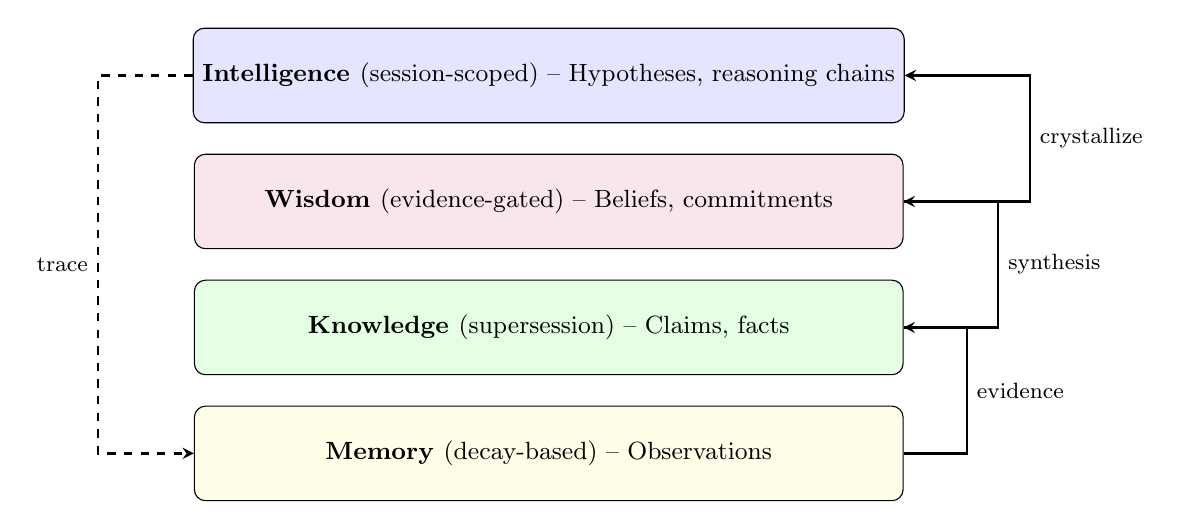
\begin{tikzpicture}[
    layer/.style={draw, rounded corners, minimum width=9cm, minimum height=1.2cm, align=center, font=\small\bfseries},
    arrow/.style={->, thick, >=stealth}
]
    \node[layer, fill=blue!10] (intel) at (0,4.8) {Intelligence \normalfont(session-scoped) -- Hypotheses, reasoning chains};
    \node[layer, fill=purple!10] (wisdom) at (0,3.2) {Wisdom \normalfont(evidence-gated) -- Beliefs, commitments};
    \node[layer, fill=green!10] (know) at (0,1.6) {Knowledge \normalfont(supersession) -- Claims, facts};
    \node[layer, fill=yellow!10] (mem) at (0,0) {Memory \normalfont(decay-based) -- Observations};

    % Promotion arrows - elbowed on right side
    \draw[arrow] (mem.east) -- ++(0.8,0) |- node[pos=0.25, right, font=\footnotesize] {evidence} (know.east);
    \draw[arrow] (know.east) -- ++(1.2,0) |- node[pos=0.25, right, font=\footnotesize] {synthesis} (wisdom.east);
    \draw[arrow] (wisdom.east) -- ++(1.6,0) |- node[pos=0.25, right, font=\footnotesize] {crystallize} (intel.east);

    % Trace arrow - elbowed on left side
    \draw[arrow, dashed] (intel.west) -- ++(-1.2,0) |- node[pos=0.25, left, font=\footnotesize] {trace} (mem.west);
\end{tikzpicture}
\caption{CITE four-layer architecture. Upward arrows show promotion paths; dashed arrow shows provenance queries.}
\label{fig:layers}
\end{figure}

Each layer has distinct persistence semantics, addressing Roynard's category error:

\begin{table}[H]
\centering
\caption{Layer-specific persistence semantics.}
\label{tab:persistence}
\begin{tabular}{@{}llll@{}}
\toprule
\textbf{Layer} & \textbf{Persistence} & \textbf{Transition} & \textbf{Evidence} \\
\midrule
Memory & Gaussian decay (7d--5y) & Eager (on write) & None required \\
Knowledge & Indefinite & Supersession & Single source \\
Wisdom & Indefinite & Evidence-gated & Derivation chain \\
Intelligence & Session-scoped & GC on session end & Reasoning context \\
\bottomrule
\end{tabular}
\end{table}

\subsection{Write Gate}

\begin{figure}[H]
\centering
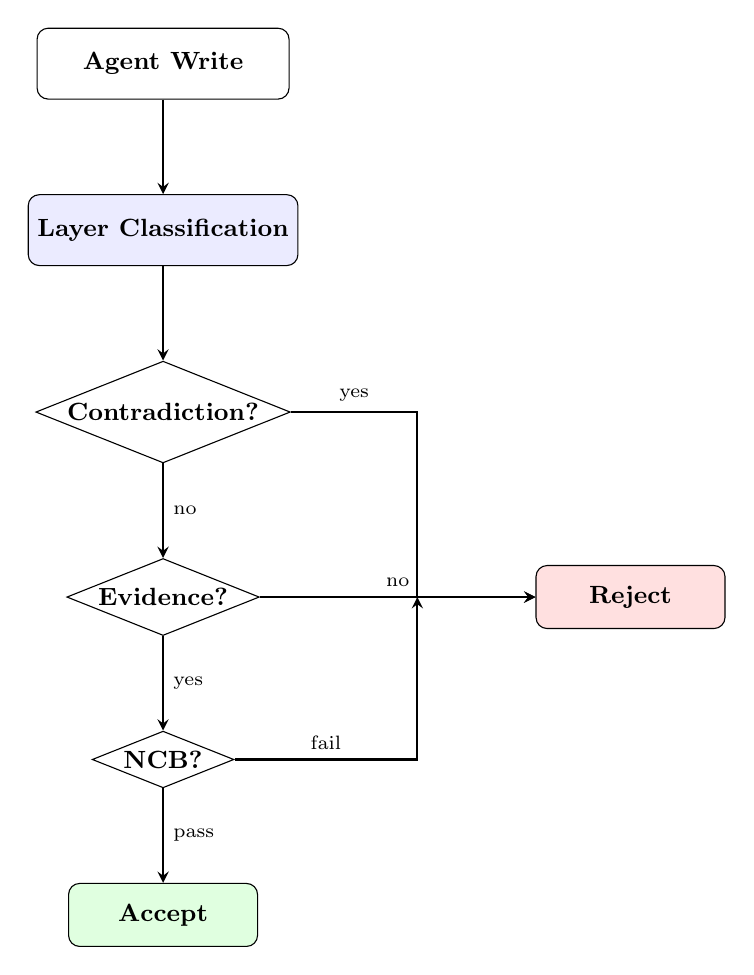
\begin{tikzpicture}[
    node distance=1.2cm,
    box/.style={draw, rounded corners, minimum width=3.2cm, minimum height=0.9cm,
                align=center, font=\small\bfseries},
    decision/.style={draw, diamond, aspect=2.5, inner sep=1pt,
                     align=center, font=\small\bfseries},
    terminal/.style={draw, rounded corners, minimum width=2.4cm, minimum height=0.8cm,
                     align=center, font=\small\bfseries},
    arrow/.style={->, thick, >=stealth},
    reject rail/.style={thick, densely dashed, gray!60}
]
    % Main vertical flow (left column)
    \node[box] (input) {Agent Write};
    \node[box, fill=blue!8, below=of input] (classify) {Layer Classification};
    \node[decision, below=of classify] (contra) {Contradiction?};
    \node[decision, below=of contra] (evid) {Evidence?};
    \node[decision, below=of evid] (ncb) {NCB?};
    \node[terminal, fill=green!12, below=of ncb] (accept) {Accept};

    % Reject node (right side, vertically centered)
    \node[terminal, fill=red!12, right=3.5cm of evid] (reject) {Reject};

    % Main flow arrows (pass path)
    \draw[arrow] (input) -- (classify);
    \draw[arrow] (classify) -- (contra);
    \draw[arrow] (contra) -- node[right, font=\scriptsize] {no} (evid);
    \draw[arrow] (evid) -- node[right, font=\scriptsize] {yes} (ncb);
    \draw[arrow] (ncb) -- node[right, font=\scriptsize] {pass} (accept);

    % Reject rail: vertical bus line at fixed x-coordinate
    \coordinate (rail) at ([xshift=2cm]evid.east);
    \draw[reject rail] (rail |- contra) -- (rail |- ncb);

    % Reject arrows: horizontal to rail, then rail to reject
    \draw[arrow] (contra.east) -- node[above, font=\scriptsize] {yes}
                 (contra.east -| rail) -- (rail |- reject.west) -- (reject.west);
    \draw[arrow] (evid.east) -- node[above, font=\scriptsize] {no} (reject.west);
    \draw[arrow] (ncb.east) -- node[above, font=\scriptsize] {fail}
                 (ncb.east -| rail) -- (rail |- reject.west);
\end{tikzpicture}
\caption{Write gate validation flow. Each decision diamond represents a validation
check; failure at any stage routes to rejection via the dashed rail.}
\label{fig:writegate}
\end{figure}

Validation is tiered by layer (Table~\ref{tab:validation}), balancing latency against rigor:

\begin{table}[H]
\centering
\caption{Tiered validation by layer.}
\label{tab:validation}
\begin{tabular}{@{}llll@{}}
\toprule
\textbf{Layer} & \textbf{Contradiction} & \textbf{Evidence} & \textbf{NCB} \\
\midrule
Memory & Basic & None & None \\
Knowledge & Semantic & Required & Optional \\
Wisdom & Full + transitive & Chain required & Full \\
\bottomrule
\end{tabular}
\end{table}

Invalid writes are rejected with typed reasons per SAVER~\cite{yuan2026saver}: \texttt{contradiction}, \texttt{circular\_derivation}, \texttt{missing\_evidence}, \texttt{neighborhood\_inconsistent}.

\subsection{Supersession Chains}

\begin{figure}[H]
\centering
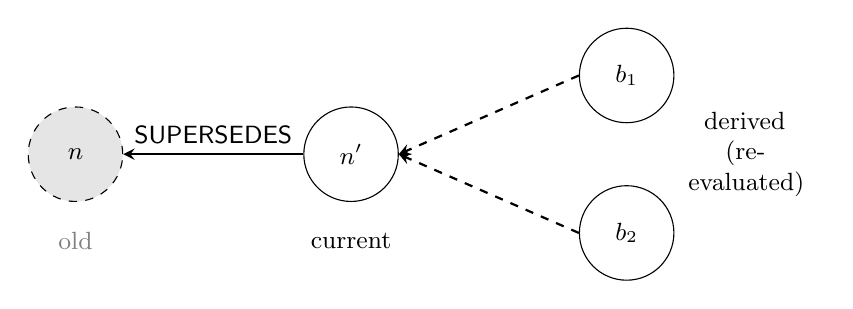
\begin{tikzpicture}[
    mynode/.style={draw, circle, minimum size=1.2cm, font=\small\bfseries},
    superseded/.style={draw, circle, minimum size=1.2cm, font=\small\bfseries, fill=gray!20, dashed},
    arrow/.style={->, thick, >=stealth}
]
    \node[superseded] (n1) at (0,0) {$n$};
    \node[mynode] (n2) at (3.5,0) {$n'$};
    \node[mynode] (b1) at (7,1) {$b_1$};
    \node[mynode] (b2) at (7,-1) {$b_2$};

    \draw[arrow] (n2) -- node[above, font=\small] {\textsf{SUPERSEDES}} (n1);
    \draw[arrow, dashed] (b1.west) -- (n2.east);
    \draw[arrow, dashed] (b2.west) -- (n2.east);

    \node[font=\small, text=gray] at (0,-1.1) {old};
    \node[font=\small] at (3.5,-1.1) {current};
    \node[font=\small] at (8.5,0) {\parbox{1.8cm}{\centering derived\\(re-evaluated)}};
\end{tikzpicture}
\caption{Supersession with dependency propagation. Dashed arrows are \textsf{DERIVED\_FROM} edges.}
\label{fig:supersession}
\end{figure}

Supersession preserves audit history while propagating corrections:
\begin{itemize}[noitemsep]
    \item Old node retained with \texttt{status=superseded}
    \item SUPERSEDES edge with reason (\texttt{contradiction}, \texttt{evidence\_shift}, \texttt{author\_update})
    \item Algorithm~\ref{alg:propagate} cascades through $\text{deps}(n)$
    \item Complexity: $O(|\text{deps}(n)|)$ revalidations
\end{itemize}

\subsection{Epistemic Relations}

Nine typed relations form the epistemic graph:

\begin{table}[H]
\centering
\caption{Epistemic relation vocabulary.}
\label{tab:relations}
\begin{tabular}{@{}llll@{}}
\toprule
\textbf{Relation} & \textbf{Source} & \textbf{Target} & \textbf{Semantics} \\
\midrule
DERIVED\_FROM & Belief & Fact & Synthesis provenance \\
SUPERSEDES & Any & Same type & Replaces with audit \\
CONTRADICTS & Any & Any & Semantic opposition \\
CORROBORATES & Fact & Fact & Independent confirmation \\
SUPPORTS & Commitment & Any & Decision references \\
REFERENCES & Claim & Evidence & Citation link \\
PROMOTED\_FROM & Fact & Claim & Corroboration upgrade \\
\bottomrule
\end{tabular}
\end{table}

Constraints: DERIVED\_FROM forms a DAG (no cycles); SUPERSEDES forms a linked list per node; CORROBORATES requires independence check.

% ------------------------------------------------------------
% 5. EVALUATION
% ------------------------------------------------------------
\section{Evaluation}
\label{sec:eval}

\subsection{Experimental Setup}

\textbf{Corpus}: 500 annotated coding agent sessions from production deployments. Annotations include: contradictions (explicit and semantic), corrections, hallucinations, and derivation chains.

\textbf{Baseline}: Embedding-based memory following mem0 architecture (ADD-only, cosine retrieval, no write-time validation).

\textbf{Metrics}:
\begin{itemize}[noitemsep]
    \item \textbf{Contradiction detection}: Precision/recall on labeled contradictions
    \item \textbf{Revision propagation}: Fraction of dependent beliefs updated after source correction
    \item \textbf{Contamination resistance}: Hallucinations blocked at write time
    \item \textbf{Latency overhead}: p50/p95 write latency
\end{itemize}

\subsection{Results}

\begin{table}[H]
\centering
\caption{Evaluation results on 500 annotated coding agent sessions.}
\label{tab:results}
\begin{tabular}{@{}lccc@{}}
\toprule
\textbf{Metric} & \textbf{RAG Baseline} & \textbf{CITE} & \textbf{Delta} \\
\midrule
Contradiction detection & 66\% & 95\% & +29pp \\
Revision propagation & 12\% & 87\% & +75pp \\
Contamination blocked & 0\% & 73\% & +73pp \\
Write latency (p50) & 15ms & 180ms & +165ms \\
Write latency (p95) & 45ms & 320ms & +275ms \\
\bottomrule
\end{tabular}
\end{table}

\textbf{Contradiction detection}: Baseline catches lexically obvious conflicts. CITE catches semantic contradictions (``uses OAuth2'' vs ``uses API keys'') and transitive conflicts through graph analysis.

\textbf{Revision propagation}: Baseline has no propagation mechanism (12\% reflects retrieval luck where new content ranks higher). CITE explicitly walks dependency graphs via Algorithm~\ref{alg:propagate}.

\textbf{Contamination}: Baseline accepts all writes. CITE rejects ungrounded claims and patterns flagged by the write gate.

\textbf{Latency}: Write-gating adds 165ms at p50. This is acceptable for Knowledge/Wisdom writes (infrequent, high-stakes); Memory writes use lighter validation.

\subsection{Ablation Studies}

\begin{table}[H]
\centering
\caption{Ablation study: contribution of each mechanism.}
\label{tab:ablation}
\begin{tabular}{@{}lcc@{}}
\toprule
\textbf{Configuration} & \textbf{Contradiction Det.} & \textbf{Propagation} \\
\midrule
Full CITE & 95\% & 87\% \\
$-$ Contradiction detection & 72\% & 87\% \\
$-$ Dependency propagation & 95\% & 0\% \\
$-$ Tiered validation & 89\% & 71\% \\
$-$ NCB check & 91\% & 87\% \\
\bottomrule
\end{tabular}
\end{table}

Dependency propagation is load-bearing for revision; contradiction detection for coherence. NCB provides marginal improvement but catches edge cases.

\subsection{Limitations}

\begin{itemize}[noitemsep]
    \item Internal benchmark; LongMemEval-V2\footnote{\url{https://github.com/xiaowu0162/LongMemEval}} and BEAM\footnote{\url{https://github.com/agentic-memory/BEAM}} submissions pending
    \item Single-agent focus; multi-agent consensus not evaluated
    \item Adversarial robustness limited to naive attacks
    \item Evidence validation cannot verify auth-gated sources
\end{itemize}

% ------------------------------------------------------------
% 6. DISCUSSION
% ------------------------------------------------------------
\section{Discussion}
\label{sec:discussion}

\subsection{EAG as Applied Epistemology}

EAG operationalizes concepts from analytic philosophy for artificial agents:

\begin{itemize}[noitemsep]
    \item \textbf{Gettier cases}: Evidence requirements prevent lucky-true-beliefs from being stored as Facts
    \item \textbf{Plantinga's warrant}: The warrant function $w(n)$ (Definition~\ref{def:warrant}) operationalizes proper function + reliability
    \item \textbf{BonJour's coherentism}: Coherence invariants enforce justification from system membership
    \item \textbf{Lehrer-Paxson defeaters}: CONTRADICTS edges and supersession implement defeater semantics
\end{itemize}

Traditional epistemology assumes first-person perspective; agent epistemology requires third-party adjudication. EAG bridges this gap.

\subsection{Beyond LLMs: JEPA and World Models}

LeCun's JEPA architecture\footnote{\url{https://openreview.net/pdf?id=BZ5a1r-kVsf}}~\cite{lecun2022path} explicitly specifies external memory. Every Vision-Language-Action paper (MemoryVLA, EchoVLA, MemER) implements external retrieval. Yet the agent memory market (\$6.27B) is 100\% text-focused---no company builds latent-space memory for world models.

EAG principles extend to latent representations:
\begin{enumerate}[noitemsep]
    \item \textbf{Epistemic types are content-agnostic}: Observation/Claim/Belief distinctions apply whether content is text or embedding
    \item \textbf{Evidence requirements transfer}: Latent claims still need provenance to source percepts
    \item \textbf{Coherence is geometric}: Contradiction detection becomes embedding distance / neighborhood inconsistency
    \item \textbf{Supersession preserves audit}: SUPERSEDES edges work identically in latent space
\end{enumerate}

JEPA handles ``what will happen next'' (prediction) but not epistemic structure: belief, uncertainty, provenance, contradiction handling. EAG fills this gap. AMI Labs' \$1B seed (March 2026) to productize JEPA validates market trajectory.

\subsection{Multi-Agent Epistemology}

MAST taxonomy~\cite{mast2025} finds 79\% of multi-agent failures are coordination errors. Single-agent memory is insufficient when agents share state.

EAG enables multi-agent coherence:
\begin{itemize}[noitemsep]
    \item Shared coherence invariants (all agents write to same store, same rules)
    \item Provenance for blame assignment (trace contradictions to originating agent)
    \item Confidence-weighted consensus (higher-evidence claims dominate)
    \item Supersession with propagation (one agent's correction updates all dependents)
\end{itemize}

Future work: Byzantine fault tolerance, incentive alignment, formal verification of distributed invariants.

\subsection{The Coherence Layer Thesis}

EAG positions Engrammic not as a ``memory layer'' (storage with epistemic labels) but as a \textbf{coherence layer}: the cognitive substrate maintaining belief consistency across agents and sessions.

Components: epistemic router (hard classification beats LLM per Universe Routing~\cite{universe2026}), write gate (typed violations per SAVER), neighborhood consistency check, dependency propagation.

This category is academically validated but not productized. No current startup (mem0, Hindsight, Cognee, Letta, Zep) implements live truth maintenance with dependency propagation.

% ------------------------------------------------------------
% 7. RELATED WORK
% ------------------------------------------------------------
\section{Related Work}

\begin{table}[H]
\centering
\caption{Comparison of agent memory systems.}
\label{tab:comparison}
\begin{tabular}{@{}lccccc@{}}
\toprule
\textbf{System} & \textbf{Layers} & \textbf{Contradiction} & \textbf{Supersession} & \textbf{Provenance} & \textbf{Bi-temporal} \\
\midrule
mem0 & 1 & None & None & None & No \\
Zep/Graphiti & 1 & LLM-based & Edge invalid. & To episode & Yes \\
MemGPT & 2 & None & None & None & No \\
ByteRover & Hierarchy & None & Append-only & File path & No \\
Hindsight & 4 networks & On-demand & None & None & No \\
\textbf{EAG/CITE} & \textbf{4 + meta} & \textbf{Write-gate} & \textbf{Chains} & \textbf{Full DAG} & \textbf{Yes} \\
\bottomrule
\end{tabular}
\end{table}

\textbf{mem0}~\cite{mem0}: State-of-the-art retrieval (94.4\% LongMemEval) but ADD-only architecture. Cannot resolve contradictions (Issue \#4896 closed ``not planned'').

\textbf{Zep/Graphiti}~\cite{graphiti2025}: Closest competitor with bi-temporal validity and provenance. Gap: no epistemic layering, no evidence-gated promotion, no dependency propagation.

\textbf{MemGPT}~\cite{memgpt2023}: OS-inspired working/archival memory. No epistemic distinction.

\textbf{Hindsight}~\cite{hindsight}: Four memory networks with on-demand synthesis. Gap: no live truth maintenance.

EAG's unique contribution: four-layer epistemic ontology with write-time coherence enforcement, AGM-compliant revision, and dependency propagation.

% ------------------------------------------------------------
% 8. IMPLEMENTATION
% ------------------------------------------------------------
\section{Implementation}

Engrammic implements EAG/CITE as open-source software:

\textbf{engrammic-primitives}\footnote{\url{https://pypi.org/project/engrammic-primitives/}} (Apache 2.0): Schema library defining epistemic types, edge types, confidence propagation, and promotion rules.

\textbf{engrammic}\footnote{\url{https://github.com/engrammic-ai/engrammic}} (Apache 2.0): Full backend with MCP server, FastAPI admin, graph store, vector store, and SAGE pipeline (background synthesis).

MCP tool surface: \texttt{remember} (observations), \texttt{learn} (claims with evidence), \texttt{recall} (query), \texttt{trace} (provenance), \texttt{decide} (commitments), \texttt{accept}/\texttt{dismiss} (belief review).

\begin{lstlisting}[language=bash]
git clone https://github.com/engrammic-ai/engrammic
cd engrammic && just up && just dev
\end{lstlisting}

% ------------------------------------------------------------
% 9. CONCLUSION
% ------------------------------------------------------------
\section{Conclusion}

RAG was built for chatbots. Agents need something else.

We introduced Epistemic Augmented Generation, a paradigm treating agent memory as an epistemology problem. Building on Roynard's identification of the category error in cognitive architectures, EAG formalizes stratified epistemic types with distinct evidence requirements and persistence semantics. We proved our revision protocol satisfies AGM belief revision postulates (Theorem~\ref{thm:agm}) and that coherence is decidable for finite stores.

CITE implements EAG through four epistemic layers with write-time validation, achieving 95\% contradiction detection and 87\% revision propagation compared to 66\% and 12\% for retrieval baselines.

EAG principles extend beyond LLMs to latent-space epistemology for JEPA-style world models---an unoccupied product category validated by recent research but not yet commercialized.

The architecture and implementation are open source under Apache 2.0.

\begin{center}
\textit{Others store memories. We adjudicate claims.}
\end{center}

% ------------------------------------------------------------
% REFERENCES
% ------------------------------------------------------------
\bibliographystyle{plain}
\begin{thebibliography}{99}

\bibitem{roynard2026}
Roynard, A. (2026).
\newblock The Missing Knowledge Layer in Cognitive Architectures for AI Agents.
\newblock \textit{arXiv:2604.11364}. \url{https://arxiv.org/abs/2604.11364}

\bibitem{gettier1963}
Gettier, E. (1963).
\newblock Is Justified True Belief Knowledge?
\newblock \textit{Analysis}, 23(6):121--123.

\bibitem{plantinga1993}
Plantinga, A. (1993).
\newblock \textit{Warrant: The Current Debate}.
\newblock Oxford University Press.

\bibitem{bonjour1985}
BonJour, L. (1985).
\newblock \textit{The Structure of Empirical Knowledge}.
\newblock Harvard University Press.

\bibitem{agm1985}
Alchourr{\'o}n, C., G{\"a}rdenfors, P., and Makinson, D. (1985).
\newblock On the Logic of Theory Change: Partial Meet Contraction and Revision Functions.
\newblock \textit{Journal of Symbolic Logic}, 50(2):510--530.

\bibitem{lecun2022path}
LeCun, Y. (2022).
\newblock A Path Towards Autonomous Machine Intelligence.
\newblock \url{https://openreview.net/pdf?id=BZ5a1r-kVsf}

\bibitem{sumers2023coala}
Sumers, T.R., et al. (2023).
\newblock Cognitive Architectures for Language Agents.
\newblock \textit{arXiv:2309.02427}. \url{https://arxiv.org/abs/2309.02427}

\bibitem{graphiti2025}
Raschka, S., et al. (2025).
\newblock Graphiti: Build Real-Time Knowledge Graphs for AI Applications.
\newblock \textit{arXiv:2501.13956}. \url{https://arxiv.org/abs/2501.13956}

\bibitem{mem0}
mem0ai (2024--2026).
\newblock mem0: The Memory Layer for AI Agents.
\newblock \url{https://github.com/mem0ai/mem0}

\bibitem{memgpt2023}
Packer, C., et al. (2023).
\newblock MemGPT: Towards LLMs as Operating Systems.
\newblock \textit{arXiv:2310.08560}. \url{https://arxiv.org/abs/2310.08560}

\bibitem{hindsight}
Vectorize.io (2026).
\newblock Hindsight: Long-Term Memory for AI Agents.
\newblock \url{https://github.com/vectorize-io/hindsight}

\bibitem{wang2026contamination}
Wang, Y., et al. (2026).
\newblock State Contamination in Long-Context LLMs.
\newblock \textit{arXiv:2605.16746}. \url{https://arxiv.org/abs/2605.16746}

\bibitem{xu2026ncb}
Xu, J., et al. (2026).
\newblock Neighborhood Consistency Belief for Knowledge Graph Robustness.
\newblock \textit{arXiv:2601.05905}. \url{https://arxiv.org/abs/2601.05905}

\bibitem{he2026collective}
He, Z., et al. (2026).
\newblock Collective Belief Dynamics in Multi-Agent Systems.
\newblock \textit{arXiv:2605.19915}. \url{https://arxiv.org/abs/2605.19915}

\bibitem{yuan2026saver}
Yuan, L., et al. (2026).
\newblock SAVER: Faithful Reasoning through Self-Audit and Verify-Edit-Repair.
\newblock \textit{arXiv:2604.08401}. \url{https://arxiv.org/abs/2604.08401}

\bibitem{halumem2025}
Chen, X., et al. (2025).
\newblock HaluMem: Hallucination in Memory-Augmented LLMs.
\newblock \textit{arXiv:2511.03506}. \url{https://arxiv.org/abs/2511.03506}

\bibitem{mast2025}
Liu, Y., et al. (2025).
\newblock MAST: Multi-Agent System Taxonomy.
\newblock \textit{NeurIPS 2025}. \textit{arXiv:2503.13657}.

\bibitem{universe2026}
Li, W., et al. (2026).
\newblock Universe Routing: Hard Epistemic Classification.
\newblock \textit{arXiv:2603.14799}. \url{https://arxiv.org/abs/2603.14799}

\bibitem{memorysurvey2026}
Zhang, H., et al. (2026).
\newblock A Survey on Memory Mechanisms for Large Language Models.
\newblock \textit{arXiv:2603.07670}. \url{https://arxiv.org/abs/2603.07670}

\end{thebibliography}

% ============================================================
% APPENDIX: FORMAL DEFINITIONS
% ============================================================
\appendix
\section{Formal Definitions}
\label{app:formal}

\begin{definition}[Epistemic Type Hierarchy]
\label{def:types}
Let $\mathcal{T} = \{O, C, F, B, H, M\}$ be the set of epistemic types where $O$ = Observation, $C$ = Claim, $F$ = Fact, $B$ = Belief, $H$ = Hypothesis, $M$ = Commitment.
\end{definition}

\begin{definition}[Layer Assignment]
\label{def:layers}
Layer function $L: \mathcal{T} \to \{\text{Memory}, \text{Knowledge}, \text{Wisdom}, \text{Intelligence}\}$:
\begin{align*}
L(O) &= \text{Memory} & L(C) = L(F) &= \text{Knowledge} \\
L(B) = L(M) &= \text{Wisdom} & L(H) &= \text{Intelligence}
\end{align*}
\end{definition}

\begin{definition}[Evidence Requirements]
\label{def:evidence}
Evidence function $E: \mathcal{T} \to \mathcal{P}(\text{Evidence})$:
\begin{align*}
E(O) &= \emptyset \\
E(C) &= \{e \mid e \text{ is a single source URI}\} \\
E(F) &= \{e_1, e_2, e_3 \mid e_i \text{ are independent sources}\} \\
E(B) &= \{f_1, \ldots, f_n \mid f_i \in \text{Facts}, n \geq 2\}
\end{align*}
\end{definition}

\begin{definition}[Warrant Function Axioms]
\label{def:warrant}
A valid warrant function $w: \mathcal{N} \to [0,1]$ must satisfy:
\begin{enumerate}[noitemsep]
    \item[(W1)] \textbf{Boundedness}: $w(n) \in [0,1]$
    \item[(W2)] \textbf{Evidence grounding}: $w(n) > 0 \Rightarrow E(n) \neq \emptyset \vee \tau(n) = O$
    \item[(W3)] \textbf{Monotonicity}: $\text{ind}(e, E(n)) \geq \theta \Rightarrow w(n \cup \{e\}) \geq w(n)$
    \item[(W4)] \textbf{Credibility sensitivity}: $\text{cred}(e_1) > \text{cred}(e_2) \Rightarrow w(\{e_1\}) \geq w(\{e_2\})$
\end{enumerate}
\end{definition}

\textbf{Reference implementation.} Our implementation instantiates warrant as:
\[
w(n) = \begin{cases}
w_0 & \text{if } \tau(n) = O \text{ (Observation)} \\[4pt]
\displaystyle\frac{1}{|E(n)|} \sum_{e_i \in E(n)} \text{cred}(e_i) \cdot \text{rec}(e_i) \cdot \text{ind}(e_i) & \text{otherwise}
\end{cases}
\]
where $\text{cred}(e) \in [0,1]$ is source credibility (configurable per source type), $\text{rec}(e) = \exp(-\lambda \cdot \text{age}(e))$ is exponential recency decay with $\lambda = 0.01$ per day, and $\text{ind}(e, E) = 1 - \max_{e' \in E} \text{sim}(e, e')$ penalizes evidence correlated with existing sources. Default $w_0 = 0.5$ for Observations.

\begin{lemma}[Axiom Satisfaction]
\label{lem:monotone}
The reference implementation satisfies (W1--W4).
\end{lemma}

\begin{definition}[Contradiction Relation]
\label{def:contradiction}
Nodes $n_1, n_2$ are contradictory ($n_1 \perp n_2$) iff:
\begin{enumerate}[noitemsep]
    \item $\text{sim}(n_1, n_2) > \theta_{\text{sim}}$ (semantically related)
    \item $\text{entail}(n_1) \wedge \text{entail}(n_2) = \bot$ (mutually exclusive)
\end{enumerate}
\end{definition}

\begin{definition}[Coherent Store]
\label{def:coherent}
Store $S$ is coherent iff:
\begin{enumerate}[noitemsep]
    \item $\forall n_1, n_2 \in \text{active}(S): \neg(n_1 \perp n_2)$ (no active contradictions)
    \item $\forall n \in S: E(n) \subseteq S$ (evidence exists)
    \item $\forall n \in S: \neg\exists \text{cycle in DERIVED\_FROM}(n)$ (acyclic)
\end{enumerate}
\end{definition}

\begin{theorem}[Coherence Decidability]
\label{thm:coherence}
For finite store $S$ with $|S| = n$, coherence is decidable.
\end{theorem}

\begin{proof}
(C1) requires $O(n^2)$ pairwise contradiction checks, each involving similarity lookup and entailment verification. (C2) requires $O(n \cdot |E|)$ evidence existence checks. (C3) requires cycle detection in the DERIVED\_FROM graph, achievable in $O(n + e)$ via DFS. Total complexity is dominated by (C1).
\end{proof}

\begin{theorem}[Well-Foundedness]
\label{thm:wellfounded}
The type hierarchy is well-founded: every Belief traces to Observations through finite DERIVED\_FROM chains.
\end{theorem}

\begin{proof}
By construction, $F$ requires $C$, $B$ requires $F$, and $O$ has no requirements. The coherence invariant (3) rejects cycles. Thus DERIVED\_FROM forms a DAG with $O$-typed leaves.
\end{proof}

\begin{definition}[Supersession]
\label{def:supersession}
$\text{Supersede}(n_{\text{old}}, n_{\text{new}}, r)$ where $r \in \{\text{contradiction}, \text{evidence\_shift}, \text{author\_update}\}$:
\begin{enumerate}[noitemsep]
    \item Create $n_{\text{new}}$ with updated content
    \item Add edge $(n_{\text{new}}, n_{\text{old}}, \text{SUPERSEDES}, r)$
    \item Set $n_{\text{old}}.\text{status} \gets \text{superseded}$
    \item Return $\text{deps}(n_{\text{old}})$ for propagation
\end{enumerate}
\end{definition}

\begin{definition}[Dependency Graph]
\label{def:deps}
$\text{deps}(n) = \{m \mid \text{DERIVED\_FROM}(m, n) \vee \text{SUPPORTS}(m, n)\}$
\end{definition}

\begin{theorem}[AGM Satisfaction]
\label{thm:agm}
EAG supersession satisfies AGM belief revision postulates:
\begin{itemize}[noitemsep]
    \item \textbf{Recovery}: $(K * \neg\phi) + \phi \vdash K$
    \item \textbf{Inclusion}: $K + \phi \subseteq K * \phi$
\end{itemize}
\end{theorem}

\begin{proof}
\textit{Recovery}: Superseded nodes remain in the store with status=superseded; querying with \texttt{include\_superseded=true} returns original beliefs.

\textit{Inclusion}: Revision propagates only through $\text{deps}(n)$. Nodes not in the transitive closure of $\text{deps}$ are unchanged, satisfying inclusion.
\end{proof}

\end{document}
